\documentclass[12pt]{article}
\usepackage[brazil]{babel}
\usepackage[utf8]{inputenc}
\usepackage[T1]{fontenc}
\usepackage{amsmath, amssymb}
\usepackage{enumitem}
\usepackage{geometry}
\usepackage{algorithm}
\usepackage{algpseudocode}
\usepackage{graphicx}
\geometry{a4paper, margin=1.5cm}

\title{BCC325 – Prova 2\\ Problemas de Satisfação de Restrições}
\author{}
\date{}

\vspace{-1cm}

\begin{document}

\maketitle

\vspace{-2cm}

Nome:

\begin{enumerate}

    \item (1,5 pt) Considere um CSP com \( n \) variáveis, cada uma com domínio de tamanho \( d \).
    
    \begin{enumerate}[label=\alph*)]
        \item Quantas atribuições totais existem neste caso?
        \item Qual é a complexidade assintótica do algoritmo \textit{generate-and-test} em termos de número de variáveis \( n \), tamanho do domínio \( d \), e número de restrições \( e \)?
        \item Explique por que este algoritmo se torna inviável para valores grandes de \( n \).
    \end{enumerate}
    
    \item (1,5 pt) Considere as variáveis \( A, B, C \in \{1, 2, 3, 4\} \) e as restrições \( A < B \) e \( B < C \).
    
    \begin{enumerate}[label=\alph*)]
        \item Liste todas as atribuições totais possíveis.
        \item Quantas dessas atribuições satisfazem todas as restrições?
        \item Mostre como a verificação de restrições em atribuições parciais pode evitar a geração de soluções inválidas.
    \end{enumerate}

    \item (1,5 pt) Responda as questões a seguir com base no algoritmo DFS solve apresentado no Apêndice ao final desta prova.

    \begin{enumerate}[label=\alph*)]
        \item Descreva o funcionamento do algoritmo \texttt{DFS\_solver} apresentado no livro 
        \item Em que momento ocorre a verificação de restrições parciais?
        \item Justifique por que isso melhora a eficiência do algoritmo em comparação ao \textit{generate-and-test}.
    \end{enumerate}

    \item (1.5 pt) Classifique cada uma das seguintes restrições quanto à sua aridade (unária, binária ou de ordem superior) e quanto à forma de representação (intencional ou extensional):
    
    \begin{enumerate}[label=\alph*)]
        \item \( A \neq B \)
        \item \( \text{Sala}(\text{Aula1}) = \text{Sala2} \)
        \item Tabela que lista todas as combinações válidas de três variáveis
        \item \( E < A \land E < B \land E < C \land E < D \)
    \end{enumerate}

    \item (2 pts) Considere a sua implementação do backtracking para o problema de alocação de salas?
    
    \begin{enumerate}[label=\alph*)]
        \item Quais são as variáveis, domínios e restrições envolvidas?
        \item O que o código faz para garantir que as restrições sejam satisfeitas?
        \item Apresente a primeira solução completa que o seu algoritmo irá gerar?
    \end{enumerate}

    \item (2 pts) Resolva as questões a seguir nos labitintos abaixo:

    \begin{enumerate}
        \item Calcule o valor da heuística distância de Manhattan para cada casasa livre.
        \item Numere os nós expandidos pelo algoritmo A$^*$, assumindo custo unitário e heurística distância de Manhattan. Em caso de empate a ordem deve ser, cima, baixo, esquerda ou direita.
        %\item Numere os nós expandidos por uma busca gulosa utilizando distância de Manhattan até o objetivo como heurística.
        %\item Numere os nós expandidos pelo algoritmo A* usando custo e heurística de Manhattan.
    \end{enumerate}

    \begin{figure}[h]
    \centering
    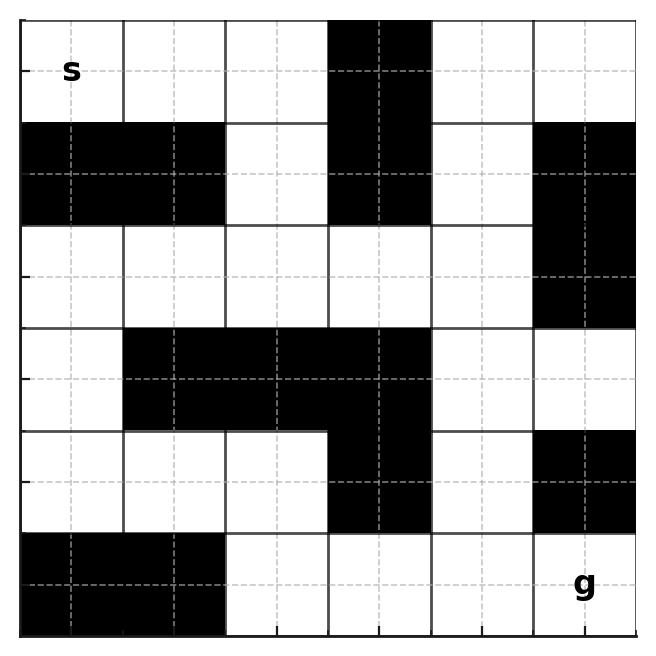
\includegraphics[width=0.4\textwidth]{labirinto.png}
    \caption{Labirinto para a heurística}
    \end{figure}

    \begin{figure}[h]
    \centering
    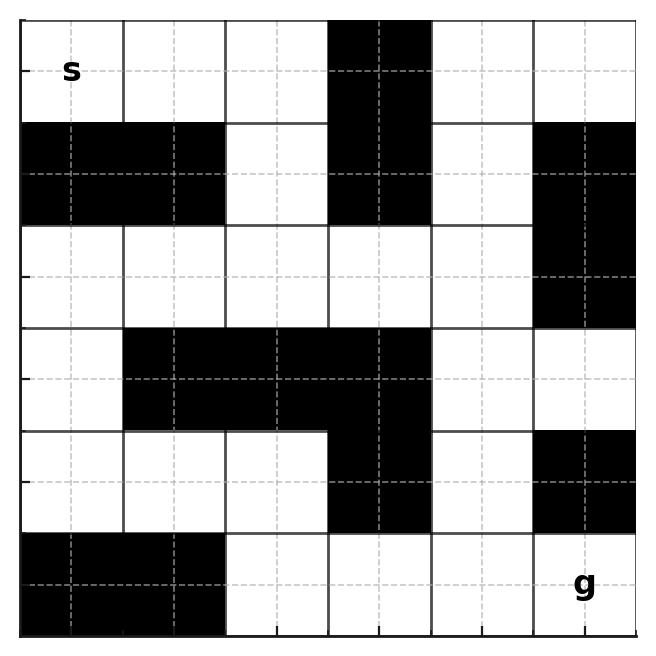
\includegraphics[width=0.4\textwidth]{labirinto.png}
    \caption{Labirinto para o A$^*$}
    \end{figure}

\end{enumerate}


\section*{Apêndice – Algoritmo \texttt{DFS\_solver}}

\begin{algorithm}[H]
\caption{\textsc{DFS\_solver}(\( V_s, C_s, \text{context} \))}
\begin{algorithmic}[1]
\State \( c_e \gets \{c \in C_s \mid c \text{ pode ser avaliado no } \text{context} \} \)
\If{\( \text{context} \) viola alguma restrição em \( c_e \)}
    \State \Return \{\}
\ElsIf{\( V_s = \{\} \)}
    \State \Return \{context\}
\Else
    \State selecione variável \( var \in V_s \)
    \State \( sols \gets \{\} \)
    \ForAll{\( val \in \text{domínio}(var) \)}
        \State \( sols \gets sols \cup \textsc{DFS\_solver}(V_s \setminus \{var\}, C_s \setminus c_e, \{var = val\} \cup \text{context}) \)
    \EndFor
    \State \Return \( sols \)
\EndIf
\end{algorithmic}
\end{algorithm}

\end{document}
